\subsection{Antagonism}\label{antagonism}

A fundamental principle in the body plan of bilaterians is the organization of movement through antagonistic pairs of effectors. Muscles, by their biological constitution, can only contract (i.e., pull) but not push. This morphological constraint necessitates the evolution of opposing pairs of muscles—flexors and extensors, abductors and adductors, pronators and supinators—that can act in reciprocal fashion to enable controlled motion \cite{Huxley1932_RelativeGrowth,Schilling2011_AntagonisticEvolution}. The bilaterian body plan, with its segmentation and bilateral symmetry, provides the structural basis for this arrangement.

At the neural level, antagonism is implemented by the canonical circuit motif of reciprocal inhibition. Sherrington’s classic work established that the activation of one muscle in a pair is accompanied by inhibition of its antagonist, ensuring coordinated and efficient movement \cite{Sherrington1906_IntegrativeAction}. This basic inhibitory scheme remains central to vertebrate and invertebrate motor control and underlies the formation of stable motor patterns.

From a biomechanical perspective, antagonistic control confers several advantages. Co-activation of antagonists allows modulation of joint stiffness, enabling both stability and compliance. Such mechanisms are critical for adaptive interaction with the environment and have inspired numerous robotic implementations of antagonistic actuators \cite{Hogan1984_ImpedanceControl,Tondu2012_McKibbenMuscle}. In biological systems, this provides the capacity not only to move but also to regulate impedance and precision.

In the context of the sensation-modulating network (SMN), antagonism is not merely a mechanical solution but also a higher-order organizational principle. Antagonistic structures encode dynamic balances: approach versus avoidance, activation versus inhibition, flexion versus extension. These embodied oppositions structure the repertoire of available action schemas and affordances, contributing to the cognitive architecture of the SMN itself \cite{Bizzi2013_MuscleSynergies}. Thus, antagonism serves as both a morphological constraint and a generative principle for embodied cognition.

\begin{figure}[htbp]
  \centering
  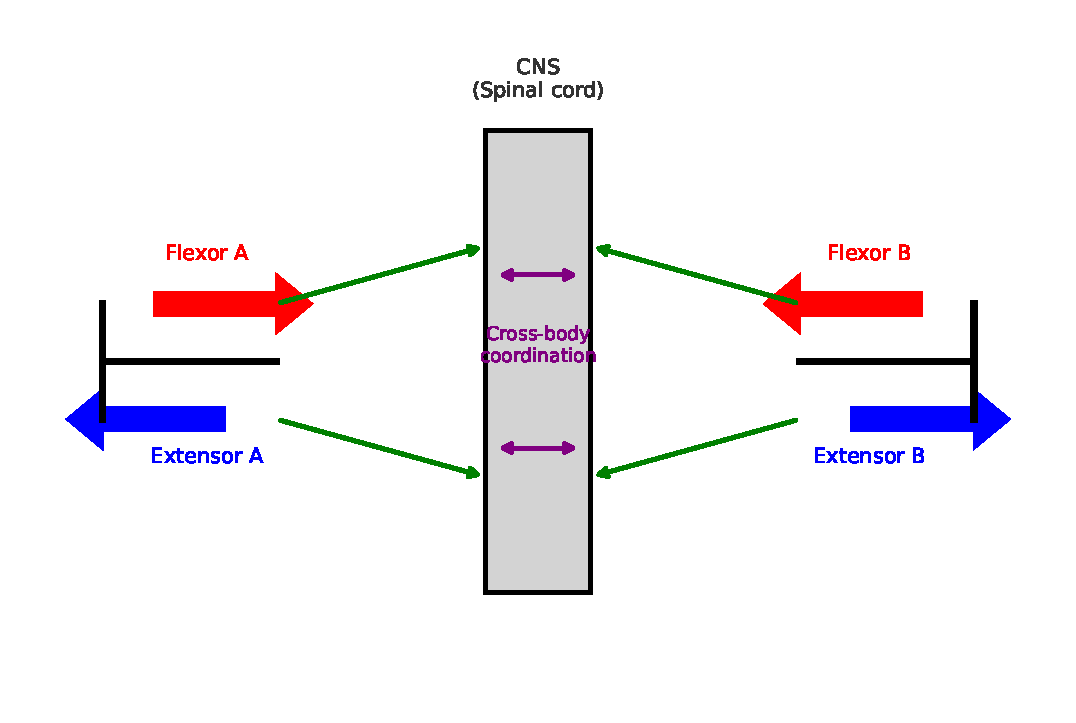
\includegraphics[width=0.8\textwidth]{graphics/smn_antagonism_bilateral_cns.pdf}
  \caption{%
    Antagonism at multiple levels of the body plan. 
    Local antagonism operates between flexor and extensor pairs within each action zone (red and blue arrows). 
    Reciprocal inhibition is mediated through central nervous system pathways (green arrows into the spinal cord). 
    Cross-body coordination (purple arrows) connects bilaterally symmetrical zones, showing how antagonism is both a morphological and neural principle.%
  }
  \label{fig:smn-antagonism}
\end{figure}
